%\title{beavtex}
\documentclass[double,12pt]{beavtex}
\usepackage{graphicx}
\usepackage{rotating} %Package added to allow the rotation of figures and chart on a page, {sidewaysfigure} command
\usepackage{tablefootnote} %Packaged added to allow footnotes in the tabular environment, use \tablefootnote command
\usepackage[polutonikogreek,english]{babel}
\newcommand{\greek}[1]{{\selectlanguage{polutonikogreek}#1}}

\title{Waves and Robots with MPC and Stuff}
\author{Daniel Fern\'{a}ndez}
\degree{Master of Science}
\doctype{Thesis}
\department{Mechanical, Industrial, and Manufacturing Engineering}
\depttype{School}
\depthead{Head}
\major{Robotics}
\advisor{Geoffrey A. Hollinger}
\submitdate{1 September 2015}
\commencementyear{2015}


\abstract{Autonomous marine vehicle decision making is an active avenue of research in the Field Robotics Community. Much of this work includes advancing underwater path planning, localization, and perception. Developments in this field can lead to cost-effective methods of deploying marine energy arrays. The purpose of this document is to summarize some of the more promising research applications as well as justify the use of autonomy in the offshore community.}


\acknowledgements{This work is supported by Department of Energy Grant number DE-EE-0006816.0000. I would like to also acknowledge...Lorem ipsum dolor sit amet, consectetur adipiscing elit. Maecenas vel eros sed mauris porttitor semper nec a orci. Nullam vestibulum mi nec condimentum posuere. Pellentesque eget diam id sapien aliquet ullamcorper. Pellentesque blandit nec lectus ut mollis. Praesent in facilisis justo. Vestibulum ante ipsum primis in faucibus orci luctus et ultrices posuere cubilia Curae; Sed eget congue leo, sed consequat libero. In rutrum malesuada nisi. Vestibulum ante ipsum primis in faucibus orci luctus et ultrices posuere cubilia Curae; Morbi sollicitudin tortor ut sem facilisis mollis.}


\begin{document}
\maketitle
\mainmatter

%-------------------------INTRODUCTION-----------------------------

\chapter{Introduction}

The increasing demand for alternative energy sources has created new opportunities in wave energy extraction. With these opportunities come new challenges; however, and much of the appeal of this constant and powerful energy source is curbed when compared to the cost of deployment and maintenance of Wave Energy Convertors (WEC). One goal of the National Northwest Marine Renewable Energy Center (NNMREC) ALFA project aims to explore new avenues to increase the cost-effectiveness of WEC maintenance by employing autonomous robotic platforms to inspect, monitor, and intervene. Field experiments are currently carried out at the NNMREC North Energy Test Site (NETS) two nautical miles off the Oregon Coast as shown in Figure \ref{fig:nets}. 

\begin{figure}[h!]
\begin{center}
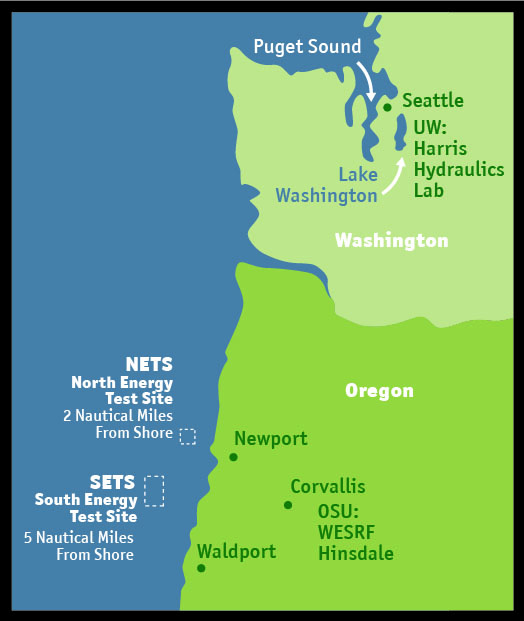
\includegraphics[width=0.5\columnwidth]{nets}
\caption{NNMREC is a partnership between the U.S. Department of Energy, Oregon State University, the University of Washington, and the University of Alaska Fairbanks. NNMREC operates and manages NETS and SETS among other facilities.}
\label{fig:nets}
\end{center}
\end{figure}

\section{Objective}

The purpose of this study is to... Lorem~\cite{petres} ipsum dolor sit amet, consectetur adipiscing elit. Sed venenatis nunc sapien. Praesent imperdiet nulla eu rutrum venenatis. Fusce rhoncus urna a nunc semper, non venenatis lorem tempor. Cras sollicitudin eget velit eu venenatis. Mauris imperdiet pretium massa sed dapibus. Nunc ipsum ipsum, porttitor ut urna ut, pretium feugiat leo. Nunc magna enim, facilisis a porttitor eget, elementum ac turpis. Quisque et gravida justo. Etiam vulputate quam at commodo suscipit. Vivamus ut adipiscing tortor. Phasellus quis dolor et mi hendrerit sollicitudin. 

Cras dapibus congue mauris, et imperdiet magna pellentesque non. Sed venenatis adipiscing quam ut placerat. Praesent imperdiet dignissim cursus. Phasellus mattis nibh vitae semper pellentesque. Lorem ipsum dolor sit amet, consectetur adipiscing elit. Sed dignissim tellus id adipiscing tempus. Aenean posuere malesuada rhoncus. Ut quis elit eros.


\chapter{Background}

\section{Wave Energy}

The world's oceans can produce close to 2 TW -- roughly twice the current global usage -- of usable wave energy \cite{falnes}. Compared to solar and wind sources, wave energy is relatively predictable and available on a constant basis. Some challenges facing wave energy extraction are: poor scaled economics, a high rate of infrastructure wear, and unclear effects to the coastal geomorphology. All of these are active areas of research in the field.

According to Linear Wave Theory (LWT), the energy in one water wavelength is the sum of its potential and kinetic energies \cite{D&D}. After some derivation it is reduced to: 
\begin{equation}
E_L = 1/8 \rho g H^2 L
\end{equation}
Though simplified, this relationship illustrates a noteworthy point that neither the average potential nor kinetic energy per unit area depends on water depth, but instead is simply proportional to the squared waveheight term, H. The rate at which energy is transferred is the energy flux, and for LWT it is the rate at which work is being done by change in energy density of a fluid over a vertical face \cite{D&D}.

Wave energy conversion as a whole is a young industry, and as such, as many competing converter designs. Point absorbers are small devices that freely oscillate at the water surface, expanding and contracting some working fluid. An attenuator is a jointed body that floats parallel to the wave direction, generating energy from the relative motion at the joint. An Oscillating Water Column (OWC) device uses differences in atmospheric pressure to force trapped air through a turbine as it is forced out by wave action \cite{falnes}. The arrays to be deployed at NNMREC test sites are yet to be determined; however, they will all require similar mooring and anchor systems. Thus, immediate robotic testing for ALFA is within reason.

\section{Wave Forces in the Water Column}

\section{Wave Prediction Models}

\section{Model Predictive Control} 


%------------------------LIT REVIEW--------------------------------

\chapter{Literature Review}

\section{Marine Platforms}

Underwater vehicles can be classified into one of two generic categories: manned and unmanned vehicles. Unmanned Underwater Vehicles (UUV) are often labeled as synonymous with Autonomous Underwater Vehicles (AUV). This can be misleading as it is not an accepted standard. For the scope of this paper, the term AUV will be used for an untethered unmanned vehicle. The term Remotely Operated Vehicle (ROV) will be used to describe a tethered manned vehicle whose operation may or may not be tele-operated \cite{ROV}. No manned vehicles will be discussed.

The term ``glider'' may on occasion be used to describe a type of AUV. Gliders such as the Slocum shown in Figure \ref{fig:slocum} are designed to move efficiently through the water column by changing their weight \cite{bachmayer}. Successive pitch adjustments up and down result in a sawtooth profile with no external propulsion.

\begin{figure}[h!]
\begin{center}
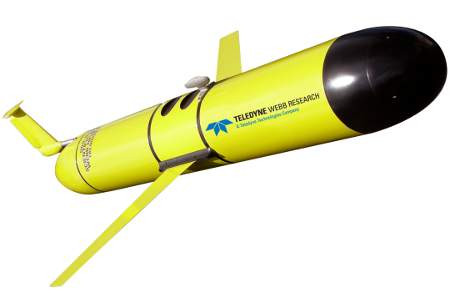
\includegraphics[width=0.5\columnwidth]{slocum}
\caption{A Webb Research Slocum Glider. This AUV uses only a buoyancy differential and small attitude adjustments to achieve an ultra low-wattage (0.5-1.0 Watts) and long range mission profile.}
\label{fig:slocum}
\end{center}
\end{figure}

\section{Path Planning}
One of the more active areas of research in Field Robotics is optimal path planning. Planning methods combine discretized graphs, heuristic search, and dynamic programming which, when properly balanced, give close to optimal results at a reduced computational cost \cite{lavalle}. Underwater robotics is no different, albeit with its own unique challenges. One such challenge is vehicle localization in an environment absent GPS and long range wireless transmissivity. Relative measurements can be provided by onboard sensors and corrected for uncertainty. The method employed by Galceran et al. \cite{galceran} uses a 2-phase approach to produce a sonar generated bathymetric map. In it, a standard mow-the-lawn pattern is employed using an \textit{a priori} input to distinguish the seafloor into regions of low and high slope with a user-defined gradient. Once the map is split, the planar regions are covered exhaustively with a path generated in a Travelling Salesman (TSP) manner while high-sloped regions are ignored as obstacles. After, the high-slope regions can then be covered with a slicing algorithm, where the vehicle travels in a spiral fashion along greedily linked adjacency points. Localization is provided by an onboard Doppler Velocity Log (DVL) and Inertial Measurement Unit (IMU) while submerged, and GPS while at the surface. The vehicle path is adaptively replanned for uncertainty using a Stochastic Trajectory Optimization Motion Planning (STOMP) method to account for errors from its ground true position.

Some sampling techniques are analysed in \cite{mora} and compared with a prioritized cost-evaluation function. This function balanced three mission metrics: collected samples, energy consumption, and mission duration. Their results showed that in almost all sampling scenarios, a stratified random spiral pattern is the most effective sampling method. This method is similar to that employed by the GIRONA 500 AUV in \cite{galceran} to measure high-slope areas. In \cite{binney}, an informed path planning method is applied to a Slocum Glider, where the vehicle can maximize user-weighted information gain while avoiding high-traffic areas during specific time windows, traveling there only at night. The recursive algorithm uses a “diminishing returns” approach, rewarding travel to unexplored nodes. This work is expanded upon in \cite{binneyB&B} with a Branch and Bound (B\&B) search algorithm which chooses the best path for the glider based on a probabilistic model of measurement quality expected. This model is a generalization of the Gaussian probability distribution of \cite{GP} of whether a point in space adds to the ``informativeness'' of the scalar field being sampled. The specific goal of the algorithm is to find the path which minimizes the average variance reduction in the Gaussian Process (GP) model. The results show that though exhaustive search is optimal in an infinite horizon, this is not computationally efficient. By limiting the horizon and using B\&B to keep track of these searches, costs are cut dramatically. The authors also suggest using a heuristic to increase the lower bound more quickly.

Another interesting path-planning solution for a Slocum Glider is presented by Smith et al. in \cite{smithglider}. Here, the unique glider dynamics are considered in creating an algorithm which will traverse areas of high interest, adjust its sampling density accordingly, and avoid areas of strong and/or variable currents. Unlike other underwater vehicles, a glider performs poorly when running a traditional mow-the-lawn pattern due to poor navigational accuracy and reliance on dead reckoning. Instead, a glider “flies” in a zigzag pattern, one where its sampling density is directly related to its pitch angle. In this approach, an expert-imported interest domain and current data from a Regional Ocean Modeling System (ROMS) feed are inputted to the algorithm and subjected to field trials. The most usable results were those of a trial in the Southern California Bight (SCB), where the algorithm scored 20\% better than a precomputed trajectory. Simulator results on an A* derivative are carried out by Fern\'{a}ndez-Perdomo et al. in \cite{fernandez} show that accounting for ROMS-generated ocean currents in path generation leads to reduced overall travel times.

Path optimization is a pivotal aspect of robotic path planning. In general, the amount of information gain should be maximized while considering some cost function, often times the mission duration. This approach is shown in \cite{smithtracking} where a sampling path is designed to track a specific oceanographic point of interest and update accordingly. Expanding upon this in \cite{smithfront}, Smith et al. applied an Ecomapper AUV to autonomously track and move along Oceanographic Fronts. These fronts serve as gradients in the ocean water properties and are directly affiliated with plankton populations. The algorithm employed uses a prior estimation of the front locations and then aims to sample the front by repeatedly crossing the AUV through it. New waypoints are generated as the front status is ascertained and compared to GPS readings. The next waypoint is generated to either cross the front again or continue searching, whichever is more efficient. The results showed that preplanned routes were shorter than the adapted routes. This is because the algorithm tended to work conservatively, using a cubic spline which overestimated the front curvature. Otherwise, the vehicle moved well along waypoint contours.

Another efficient path planning approach is the hybrid Fast Marching (FM) method, or FM*, employed in \cite{petres}. This approach uses an A* search heuristic to find a continuous path through a discretized, static world, converting meshes to save on computation time. In addition, the algorithm accounts for the vehicle kinematics and adapts the trajectory for underwater currents. The simulator results are promising but presented without any field trials, listing that as an avenue for future work. 

\section{Localization}
A central focus in greater robotics is the Simultaneous Localization And Mapping, or SLAM problem. This arises when a robot either does not have access to a map of its environment or it cannot determine its position in an \textit{a priori} map \cite{prob}. SLAM techniques attempt to generate a map of the environment while simultaneously localizing a robot within it. It is a difficult and costly problem to solve as maps and relative positions must be estimated throughout. 

Efficient area coverage and good SLAM performance in navigation; however, are conflicting objectives. To provide efficient coverage, redundant overlapping trajectories need to be minimized while still accounting for vehicle/sensor ``drift'' over time. In \cite{kim}, Kim and Eustice introduce an active visual SLAM method of perception-driven navigation which balances exploration and revisitation using a reward function. They used a visual saliency method to compute image scores and schedule revisits accordingly. The saliency score assumes that visual SLAM treats images unequally, a fair assumption especially underwater, where the spatial distribution of desired features is not consistently apparent. As a set of waypoints is generated, a reward for that path is computed based on its overall saliency. The reward is then compared with the cost of travel and the robot then moves. 

Results for \cite{kim} are presented in a simulator and through HAUV field trials in a ship hull inspection role for the \textit{SS Curtiss}. The AUV plans paths autonomously and then revisits waypoints to close loops and minimize navigation uncertainty by comparing features at its ``drifted'' position with prior features. This uncertainty horizon controls how opportune revisits are and directly affects the strategy cost. This work is expanded upon in \cite{chaves} where the loop-closing navigation uncertainty is probabilisticially modeled using GP regression. This approach combines sampling-based plans with information filters to quickly search many paths given a utility function. Trials were again carried out on \textit{SS Curtiss} and results were compared to \cite{kim}. The proposed method showed an improved path length with uncertainty levels similar to the ``best possible'' deterministic model.

Active SLAM as presented in \cite{kim} and \cite{chaves} is effective in a hull inspection application as it can use previously recorded features to adjust for uncertainty. In a bathymetric mapping application; however, this is not a preferred approach as the seafloor is largely featureless. In \cite{barkby}, Barkby et al. employ an efficient and featureless bathymetric SLAM with a Rao-Blackwell particle filter and GP Regression for depth uncertainty loop closures. This method overcomes feature dependency by generating a particle-based 2D depth map from successive identical point clouds of bathymetric observations. To save memory, the entire point cloud is not saved; the backtraceable trajectory of each child point is recorded to a parent map in a process called Distributed Particle Mapping (DPM). Each observed state is removed from the particle filter and tracked by a single shared extended Kalman filter. A bathymetric map can be inputted or initialized to zero. The algorithm was tested on a Sirius AUV, a JASON ROV, and a Sentry AUV at different locations, showing consistently small particle set sizes and generating similar maps to Ultra Short Base Line (USBL) data at a minimum computation time. 

\begin{figure}[h!]
\begin{center}
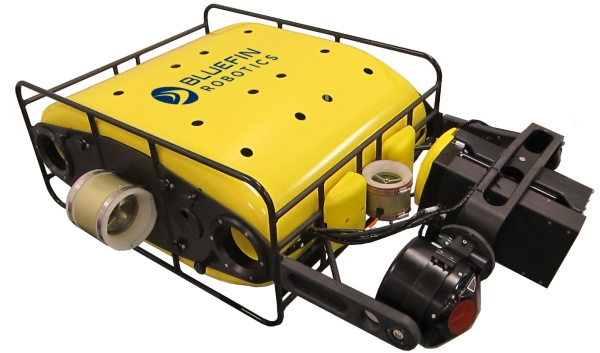
\includegraphics[width=0.5\columnwidth]{hauv}
\caption{A Bluefin Hovering Autonomous Underwater Vehicle, or HAUV, as referenced in \cite{kim} and \cite{hover}. This vehicle was used along with a Didson sonar to reconstruct the \textit{S.S. Curtiss} hull draft.}
\label{fig:hauv}
\end{center}
\end{figure}

\section{Perception}
Another active area of research in Field Robotics is interpreting real-world observations. A plethora of methods on this topic have been published, and each carries its own applied merits and detriments. In \cite{papa}, Papadopoulos et al. use a SCOUT Autonomous Surface Vehicle (ASV) with off-the shelf sensors to obtain reconstructions for partially-submerged structures in rough sea conditions. The ASV used a LiDAR Camera to collect data above the water line, where the vehicle travelled around the target in a circle, recording data in a point cloud. This data is then passed through an Iterative Closest Point (ICP) minimizing algorithm and then filtered to reconstruct the observed surface. Additionally, the vehicle used a sonar emitter to collect data below water. The results, although not novel in their approach, are still interesting in their low cost execution. Another interesting takeaway was that this method did not require a pre-computed trajectory, like SLAM techniques. This allowed the vehicle to reconstruct slow-moving structures and even watercraft. 

In addition to presenting the aforementioned path-planning techniques in \cite{galceran}, the authors also detail their surface reconstruction method. In it, the sonar sensor populates a triangular mesh grid with points and normal obtained as gradient samples of a minimized volumetric indicator function. When minimized, the surface can then be extracted as a zero level set using surface contours. The normals are estimated using a Hoppe Method, which fits a plane in a local k-neighborhood around each point. Another interesting approach is outlined in \cite{dunbabin}, where the authors attempt to use a Starbug AUV as a “mule” to transfer data from non-communicating submerged sensor nodes. A path is plotted from node to node using a TSP solver with uncertainty and the nodes are found using computer vision. This approach looks for a specific color range and maintains the object camera center while data is up/downloaded. 

Lighting issues, camera contrast, and blurring all hinder camera operation in an underwater application. By needing only non-orthogonal captured raw camera point sets, the method devised by Campos et al. in \cite{campos} is widely applicable. The process employs Restricted Delaunay Triangulation (RDT) meshing which takes a small set of points and iteratively constructs a course-to-fine triangle surface. This is done online and is shown to be able to process corrupted point sets with loose input requirements and a low memory footprint. RDT selects the points which lie in a local neighborhood and logarithmically filters out any outliers. Any intersections between local segments is answered and generates a finalized Local Bivariate Quadric (LBQ) surface. Results are presented on a number of different multi-beam sonar experiements on sources with varying complexities and added noise sets. The method is also experimented on an optical stereo multi-view seafloor reconstruction. Though the algorithm struggled with vertical walls at shallow observation heights, the post-processed results were still robust despite a high number of outliers.

Interpreting the novelty of each observation is equally important as making the actual observation. In \cite{girdhar}, Girdhar et al. use an online topic modeling approach to compute the “surprise” score of an observation. Applied, a vehicle could explore an environment as a tourist would explore a new city: stop and observe if new, move along if not. Using this method, an underwater robot was able to recognize and record different species of coral while having its speed controlled by mapping this “surprise” score through a sigmoid function.
 
\section{Combined Systems}
By combining these path-planning and surface reconstruction techniques, a number of useful applications similar to the bathymetric mapping in \cite{galceran} can then be performed. Another such application is modeling and inspecting the hull of a berthed ship as detailed in \cite{geoffadapt}, \cite{geoffuncertainty}, and \cite{hover}. Hollinger et al. seek to construct closed 3D meshes from sonar-induced point clouds and measure the uncertainty on the closed mesh using non-parametric Bayesian regression. Specifically, the method applys a GP implicit surface with augmented input vectors for uncertainty and use a probabilistic path planner to minimize uncertainty while maximizing the mesh coverage. Here, the surface uncertainty is a generalization of the probability distribution of whether a point in space is in fact on the mesh surface. The input vectors can be supplied in various ways; in this paper, they are supplied by way of an initial coarse survey over the ship hull. \cite{hover} uses a similar Poisson surface reconstruction method for sonar imaging and 3D mesh modeling as \cite{geoffadapt}. The path planning is slightly different; however, as it uses a computationally inexpensive TSP/RRT solver to create a probabilistically complete and asymptotically optimal solution.

In \cite{geoffmapping}, Hollinger and Sukhatme apply their prior work in \cite{geoffadapt} and \cite{geoffuncertainty} to a feature mapping role. Here, a YSI EcoMapper AUV is used to dive Puddingstone Lake, CA and generate dense bathymetric maps using a sidescan sonar. Their approach again models uncertainty in the form of a GP, where the actively planned path seeks to maximally reduce the variance while accounting for onboard budget constraints. Paths are then selected greedily. In addition, they allow for dives to be adaptively replanned as more information becomes available to the vehicle. These re-planned dives are computed offboard and communicated to the vehicle after a human operator checks for safety. Results show that their planned path shows substantial improvement over standard lawnmower patterns and show limited improvement when adaptively re-planning, showing an 8\% reduction in uncertainty over the first re-planning cycle and no improvement over the second re-planning cycle. They cite reducing the computational cost of adaptivity as an avenue of future work.

\begin{figure}[h!]
\begin{center}
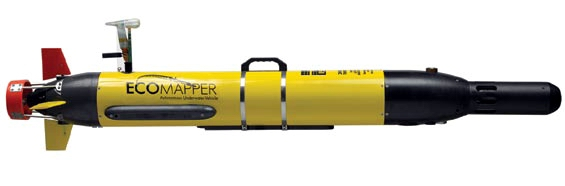
\includegraphics[width=0.5\columnwidth]{eco}
\caption{A YSI EcoMapper AUV as referenced in \cite{smithfront} and \cite{geoffmapping} which along with a side-scanning sonar was used to construct dense bathymetric maps of the floor of Puddingstone Lake, CA.}
\label{fig:eco}
\end{center}
\end{figure}

Ocean currents often lead to untethered AUV's such as the Slocum suffering from increasing positional uncertainty over their mission profiles. If the vehicle is equipped with a DVL and the water depth is shallow enough (~<200m), then localization becomes significantly more trivial. In the mid-water column, which is the submerged space outside the DVL bottom lock range, the vehicle relies solely on dead reckoning to localize itself. In \cite{medagoda}, Medagoda et al. propose a novel method of using a vehicle's DVL as an Acoustic Doppler Current Profiler (ADCP) to instead measure water current relative to the vehicle. Applied, this can constrain the positional error to the initial current velocity uncertainty at the sea surface. In addition, if bottom lock is achieved at any point, the velocity history is constrained to 2\greek{σ} by fusing the dead reckon and current estimates. The method is validated using field data from a Sentry AUV, where DVL and USBL inputs to the AUV are blacked out while the vehicle performs a series of lawnmower patterns. Results show that with no prior info about the true water currents, positional errors with the USBL are within 600m at 17km (3.5\%) for 8 hours and 8km at 84km (9.5\%) at 20 hours. 

Onboard vehicle sensors are often used to compensate for accumulated position error. Another active avenue for autonomy in marine robotics; however, is the use of in situ data to allow for active replanning and to guide sampling decisions. A model is described in \cite{smithmeas} which uses a Wave Glider AUV. Its goal is to learn a linear predictive regression model which inputs environment data to predict glider speed. The appeal is to use this data for better offline objective planning. Their results concluded that the dominant contributors to glider speed predictions were the significant wave height and peak wave period. This is not surprising, as they are the dominant contributors to orbital velocities in the surf zone \cite{D&D}. Their work is expanded upon in \cite{ngo} using a GP-based approach to mixed results.

This approach is expanded upon in \cite{hitz} where Hitz et al. attempt to use the onboard sensor data as the adaptive path planned threshold criteria. They employ a receding horizon path planner to reduce the uncertainty around this specific criteria, which generates optimal sampling paths connecting highlighted sites along a user-defined vertical transect plane. The uncertainty model is GP-derived and uses no \textit{a priori} information on initialization. They provide simulator and field results on an ASV tracking toxic cyanobacteria. The vehicle traveled 18km and showed reduced uncertainties of 68\% when compared to non-adaptive techniques.

Though there is no ROV involved, the multi-robot approach in \cite{eich} proposes a novel solution to the ship-hull inspection problem. The three robots, a small quadcopter and two magnetic crawlers, employ a three phase approach. First, the Pelican Quadrotor gives a top level scan of the interior of a cargo bay using computer vision to find the more compromised areas. Second, a lightweight magnetic robot crawls along the walls using a Monte Carlo localization method and an onboard camera to inspect the coating corrosion and any cracks in the hull. Finally, the heavier Magnetic Autonomous Robotic Crawler (MARC) crawls along the walls with a similar localization method but uses an ultrasound sensor to measure any irregularities in the material thickness of the vessel. The work is preliminary and many locomotion, point cloud, and multi-agent improvements are suggested, but is otherwise an interesting solution, especially if paired with an outer hull-inspecting ROV.

A novel multi-robot approach is presented in \cite{leonard} where a group of ten Slocum and Spray gliders are used to autonomously sample an area for oceanographic data. The different gliders have different sampling profiles; the Spray gliders patrol the outside loop of a rectangle while the Slocum gliders make three loops through the inside of it. Paths are generated to maintain equal intervehicle spacing within each loop, with gliders adaptively shortening or expanding as necessary. The algorithm also can adapt for an adjusted number of gliders within each loop. Results show that the system provided excellent coverage of the area while maintaining relatively good vehicle spacing, which further improved the sampling coverage. Strong currents were found to be an issue, but that the system adapted reasonably well. 


%-------------------MATERIALS & METHODS--------------------------

\chapter{Methods}

\section{Primary Methods}

Lorem ipsum dolor sit amet, consectetur adipiscing elit. Sed venenatis nunc sapien. Praesent imperdiet nulla eu rutrum venenatis. Fusce rhoncus urna a nunc semper, non venenatis lorem tempor. Cras sollicitudin eget velit eu venenatis. Mauris imperdiet pretium massa sed dapibus. Nunc ipsum ipsum, porttitor ut urna ut, pretium feugiat leo. Nunc magna enim, facilisis a porttitor eget, elementum ac turpis. Quisque et gravida justo. Etiam vulputate quam at commodo suscipit. Vivamus ut adipiscing tortor. Phasellus quis dolor et mi hendrerit sollicitudin. 

Cras dapibus congue mauris, et imperdiet magna pellentesque non. Sed venenatis adipiscing quam ut placerat. Praesent imperdiet dignissim cursus. Phasellus mattis nibh vitae semper pellentesque. Lorem ipsum dolor sit amet, consectetur adipiscing elit. Sed dignissim tellus id adipiscing tempus. Aenean posuere malesuada rhoncus. Ut quis elit eros.


\begin{table}[ht]
\caption{Types of stuff you put in a table} % title of Table
\centering  % used for centering table
\begin{tabular}{c c} % centered columns (2 columns)
\hline\hline                        %inserts double horizontal lines
Header 1 & Header 2 \\ [0.5ex] % inserts table heading
\hline                  % inserts single horizontal line
Item 1 & something  \\ % inserting body of the table
Item 2 & something else  \\
Item 3 & more things  \\
Item 4 & and more \\
Item 5 & last thing \\ [1ex]      % [1ex] adds vertical space
\hline %inserts single line
\end{tabular}
\label{table:misc} % is used to refer this table in the text
\end{table}



\section{More Methods}

Lorem ipsum dolor sit amet, consectetur adipiscing elit. Sed venenatis nunc sapien. Praesent imperdiet nulla eu rutrum venenatis. Fusce rhoncus urna a nunc semper, non venenatis lorem tempor. Cras sollicitudin eget velit eu venenatis. Mauris imperdiet pretium massa sed dapibus. Nunc ipsum ipsum, porttitor ut urna ut, pretium feugiat leo. Nunc magna enim, facilisis a porttitor eget, elementum ac turpis. Quisque et gravida justo. Etiam vulputate quam at commodo suscipit. Vivamus ut adipiscing tortor. Phasellus quis dolor et mi hendrerit sollicitudin. 

Cras dapibus congue mauris, et imperdiet magna pellentesque non. Sed venenatis adipiscing quam ut placerat. Praesent imperdiet dignissim cursus. Phasellus mattis nibh vitae semper pellentesque. Lorem ipsum dolor sit amet, consectetur adipiscing elit. Sed dignissim tellus id adipiscing tempus. Aenean posuere malesuada rhoncus. Ut quis elit eros.


%------------------------RESULTS--------------------------------

\chapter{Results}

Lorem ipsum dolor sit amet, consectetur adipiscing elit. Fusce posuere sed magna sit amet hendrerit. Integer gravida mattis posuere. Pellentesque at libero consectetur, pulvinar augue ac, pharetra augue. Cras fermentum augue id odio rutrum, eget eleifend lectus adipiscing. Duis libero massa, rutrum eget purus eu, tempus dapibus dolor. Class aptent taciti sociosqu ad litora torquent per conubia nostra, per inceptos himenaeos. Sed aliquet fringilla odio at euismod. Etiam viverra convallis tortor, hendrerit varius nulla pharetra ac. 

Donec vitae mollis sem, non viverra arcu. Integer vel risus justo. Proin consectetur justo nisl, ut auctor mauris rhoncus id. Vestibulum eget egestas risus. Nullam eget nunc non tortor pretium rhoncus dapibus eu orci. In hendrerit velit vel turpis vulputate porttitor. Praesent commodo, neque at porta posuere, ligula ipsum euismod dolor, ac pharetra erat purus non nunc. Praesent placerat placerat fermentum. Class aptent taciti sociosqu ad litora torquent per conubia nostra, per inceptos himenaeos. Praesent volutpat, purus id molestie egestas, mauris neque accumsan tellus, vitae fermentum lorem neque a lectus. Morbi tincidunt metus dui, vitae adipiscing mauris porttitor vitae. Donec a dolor convallis, tincidunt sapien vel, malesuada lorem. Fusce a magna sit amet leo accumsan dapibus at nec tellus. Nam id erat at ligula adipiscing porttitor in semper augue. Etiam imperdiet lobortis dui, a ornare lorem vulputate vitae. 

Etiam non libero in leo egestas porta et eu nunc. Duis molestie suscipit semper. Vestibulum nec sodales odio, vestibulum sagittis lacus. Phasellus volutpat, velit in pretium malesuada, nibh magna consequat neque, in interdum magna mi at erat. In hac habitasse platea dictumst. Praesent consectetur ut lorem sagittis tempus. Ut venenatis eu mi eget sollicitudin. Praesent posuere non lorem nec lacinia. Nunc at vulputate dolor. Aliquam et dolor sit amet quam viverra condimentum vitae eu dui. Quisque pellentesque purus in tortor vehicula sollicitudin. Curabitur sit amet vehicula diam. Vivamus mauris nulla, dictum ac ipsum eget, molestie scelerisque diam. Curabitur sit amet dolor nibh. Cum sociis natoque penatibus et magnis dis parturient montes, nascetur ridiculus mus. Sed semper sed diam quis feugiat. 


\begin{equation}
MDC=\frac{3.29*\sqrt{(Bkgcpm*C_{t}*(1+\frac{C_{t}}{BkgC_{t}}))}+3.0}{2.22*E*C_{t}*V*decay*A*R*DF*I}
\label{eq:mdc}
\end{equation}
Where:

\begin{itemize}
\item $C_{t} =$ Sample count time
\item $BkgC_{t} =$ Background count time
\item $Bkgcpm =$ Background counts per minute (cpm)
\item $E =$ Counting efficiency
\item $V =$ Sample volume or weight
\item $decay =$ isotopic decay (if applicable)
\item $A =$ Isotopic abundance (if applicable)
\item $R =$ Recovery (if applicable)
\item $DF =$ Dilution factor for liquid scintillation (if applicable)
\item $I =$ Additional decay or ingrowth factors (if applicable)
\end{itemize}

Lorem ipsum dolor sit amet, consectetur adipiscing elit. Sed venenatis nunc sapien. Praesent imperdiet nulla eu rutrum venenatis. Fusce rhoncus urna a nunc semper, non venenatis lorem tempor. Cras sollicitudin eget velit eu venenatis. Mauris imperdiet pretium massa sed dapibus. Nunc ipsum ipsum, porttitor ut urna ut, pretium feugiat leo. Nunc magna enim, facilisis a porttitor eget, elementum ac turpis. Quisque et gravida justo. Etiam vulputate quam at commodo suscipit. Vivamus ut adipiscing tortor. Phasellus quis dolor et mi hendrerit sollicitudin. 

Cras dapibus congue mauris, et imperdiet magna pellentesque non. Sed venenatis adipiscing quam ut placerat. Praesent imperdiet dignissim cursus. Phasellus mattis nibh vitae semper pellentesque. Lorem ipsum dolor sit amet, consectetur adipiscing elit. Sed dignissim tellus id adipiscing tempus. Aenean posuere malesuada rhoncus. Ut quis elit eros.


\pagebreak[4]

\begin{figure}
\begin{center}
	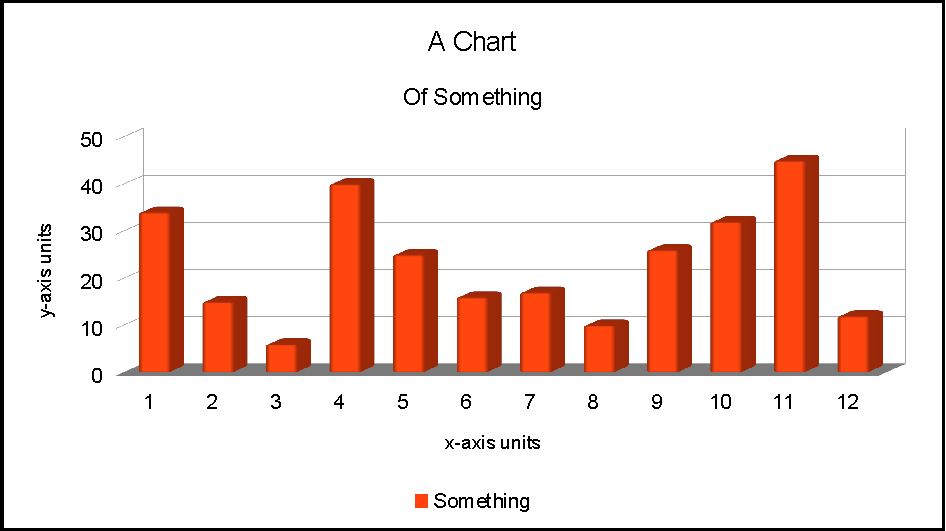
\includegraphics[width=14cm]{chart.pdf}
	\caption{A Chart.}
	\label{fig:chart}
	\end{center}
\end{figure}

\pagebreak[4]

\begin{sidewaysfigure}[htbp]
\begin{center}
	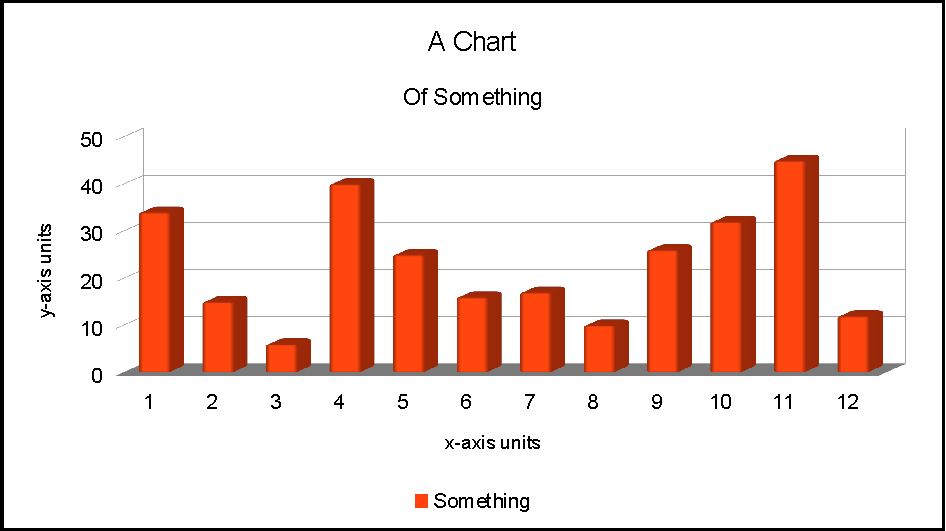
\includegraphics[width=18cm]{chart.pdf}
	\caption{Same chart, but using sidewaysfigure.}
	\label{fig:rain}
	\end{center}
\end{sidewaysfigure}


%-----------------------DISCUSSION--------------------------------

\chapter{Discussion}

\section{First Subsection}

Lorem ipsum dolor sit amet, consectetur adipiscing elit. Fusce posuere sed magna sit amet hendrerit. Integer gravida mattis posuere. Pellentesque at libero consectetur, pulvinar augue ac, pharetra augue. Cras fermentum augue id odio rutrum, eget eleifend lectus adipiscing. Duis libero massa, rutrum eget purus eu, tempus dapibus dolor. Class aptent taciti sociosqu ad litora torquent per conubia nostra, per inceptos himenaeos. Sed aliquet fringilla odio at euismod. Etiam viverra convallis tortor, hendrerit varius nulla pharetra ac. 

Donec vitae mollis sem, non viverra arcu. Integer vel risus justo. Proin consectetur justo nisl, ut auctor mauris rhoncus id. Vestibulum eget egestas risus. Nullam eget nunc non tortor pretium rhoncus dapibus eu orci. In hendrerit velit vel turpis vulputate porttitor. Praesent commodo, neque at porta posuere, ligula ipsum euismod dolor, ac pharetra erat purus non nunc. Praesent placerat placerat fermentum. Class aptent taciti sociosqu ad litora torquent per conubia nostra, per inceptos himenaeos. Praesent volutpat, purus id molestie egestas, mauris neque accumsan tellus, vitae fermentum lorem neque a lectus. Morbi tincidunt metus dui, vitae adipiscing mauris porttitor vitae. Donec a dolor convallis, tincidunt sapien vel, malesuada lorem. Fusce a magna sit amet leo accumsan dapibus at nec tellus. Nam id erat at ligula adipiscing porttitor in semper augue. Etiam imperdiet lobortis dui, a ornare lorem vulputate vitae. 

Etiam non libero in leo egestas porta et eu nunc. Duis molestie suscipit semper. Vestibulum nec sodales odio, vestibulum sagittis lacus. Phasellus volutpat, velit in pretium malesuada, nibh magna consequat neque, in interdum magna mi at erat. In hac habitasse platea dictumst. Praesent consectetur ut lorem sagittis tempus. Ut venenatis eu mi eget sollicitudin. Praesent posuere non lorem nec lacinia. Nunc at vulputate dolor. Aliquam et dolor sit amet quam viverra condimentum vitae eu dui. Quisque pellentesque purus in tortor vehicula sollicitudin. Curabitur sit amet vehicula diam. Vivamus mauris nulla, dictum ac ipsum eget, molestie scelerisque diam. Curabitur sit amet dolor nibh. Cum sociis natoque penatibus et magnis dis parturient montes, nascetur ridiculus mus. Sed semper sed diam quis feugiat. 

\begin{equation}
A(t)=A_{o}e^{(-\lambda t)}
\label{eq:initialeq}
\end{equation}

Then Equation~\ref{eq:initialeq} is integrated to become:

\begin{equation}
\tilde{C}=\int_0^{t}A(t)dt = \frac{A_{o}}{\lambda} (1-e^{(-\lambda t)})
\label{eq:finaleq}
\end{equation}

Where:

\begin{itemize}
\item $A(t) =$ original exponential function
\item $A_{o} =$ the peak activity at day 0 (Bq per mass or volume)
\item $\tilde{C} =$ Integrated Activity Concentration (Bq-days per mass or volume)
\item $t =$ 28 days
\item $\lambda =$ removal constant (day$^{-1}$)
\end{itemize}



\section{Another Subsection}

Lorem ipsum dolor sit amet, consectetur adipiscing elit. Fusce posuere sed magna sit amet hendrerit. Integer gravida mattis posuere. Pellentesque at libero consectetur, pulvinar augue ac, pharetra augue. Cras fermentum augue id odio rutrum, eget eleifend lectus adipiscing. Duis libero massa, rutrum eget purus eu, tempus dapibus dolor. Class aptent taciti sociosqu ad litora torquent per conubia nostra, per inceptos himenaeos. Sed aliquet fringilla odio at euismod. Etiam viverra convallis tortor, hendrerit varius nulla pharetra ac. 

Donec vitae mollis sem, non viverra arcu. Integer vel risus justo. Proin consectetur justo nisl, ut auctor mauris rhoncus id. Vestibulum eget egestas risus. Nullam eget nunc non tortor pretium rhoncus dapibus eu orci. In hendrerit velit vel turpis vulputate porttitor. Praesent commodo, neque at porta posuere, ligula ipsum euismod dolor, ac pharetra erat purus non nunc. Praesent placerat placerat fermentum. Class aptent taciti sociosqu ad litora torquent per conubia nostra, per inceptos himenaeos. Praesent volutpat, purus id molestie egestas, mauris neque accumsan tellus, vitae fermentum lorem neque a lectus. Morbi tincidunt metus dui, vitae adipiscing mauris porttitor vitae. Donec a dolor convallis, tincidunt sapien vel, malesuada lorem. Fusce a magna sit amet leo accumsan dapibus at nec tellus. Nam id erat at ligula adipiscing porttitor in semper augue. Etiam imperdiet lobortis dui, a ornare lorem vulputate vitae. 

Finally, a table with a footnote...

\begin{table}[htbp!]
\caption{Some table values}
\centering
\begin{tabular}{cccccc}
\hline\hline
 & & & & & Total \\
Sample & $A_{o}$\tablefootnote{some kind of footnote from a table, which doesn't work without the tablefootnote package} & $\lambda$ & $\tilde{C}$ & Something & (units) \\
\hline   \\
Item 1 & 1 & .55 & 3 & 125 & 70  \\
Item 2 & 1 & .55 & 3 & 125 & 70  \\
Item 3 & 1 & .55 & 3 & 125 & 70  \\
Item 4 & 1 & .55 & 3 & 125 & 70  \\ [1ex]
\hline
\textbf{Total} &  &  &  &  & \textbf{280} \\ [1ex]
\hline
\end{tabular}
\label{table:intake2}
\end{table}


Etiam non libero in leo egestas porta et eu nunc. Duis molestie suscipit semper. Vestibulum nec sodales odio, vestibulum sagittis lacus. Phasellus volutpat, velit in pretium malesuada, nibh magna consequat neque, in interdum magna mi at erat. In hac habitasse platea dictumst. Praesent consectetur ut lorem sagittis tempus. Ut venenatis eu mi eget sollicitudin. Praesent posuere non lorem nec lacinia. Nunc at vulputate dolor. Aliquam et dolor sit amet quam viverra condimentum vitae eu dui. Quisque pellentesque purus in tortor vehicula sollicitudin. Curabitur sit amet vehicula diam. Vivamus mauris nulla, dictum ac ipsum eget, molestie scelerisque diam. Curabitur sit amet dolor nibh. Cum sociis natoque penatibus et magnis dis parturient montes, nascetur ridiculus mus. Sed semper sed diam quis feugiat.




\chapter{Conclusion}

This paper presented some of the accomplishments in the marine robotic community. These included advancements in autonomous underwater path planning, localization, and perception. Efficient path planning helps reduce overall mission cost and time by optimizing methods of navigating. Localization issues in an environment absent GPS and long range wireless transmissivity prioritize the need for well-developed SLAM techniques with minimal input. Robotic perception in the underwater domain further complicates research efforts. In addition, multi-agent research such as the multi-glider work in \cite{leonard} is an excellent demonstration of the value of autonomy in performing oceanographic monitoring.

These advancements in underwater autonomy will be pivotal in the development of offshore energy arrays, since low-cost robotic platforms inspecting, monitoring, and manipulating infrastructure can reduce deployment costs drastically. Over the course of the NNMREC ALFA project, robust algorithms for these marine platforms to support WEC's will lead to improved scaled economics and further global wave energy development. As more challenges are addressed, this will help secure wave energy extraction as the premier sustainable energy source for the 21st century.

\pagebreak

\bibliography{thesis}
\bibliographystyle{plain}

\pagebreak

\appendix

\chapter{Things}





\chapter{More Things}





\end{document}